\documentclass[a4paper]{tufte-handout}

\usepackage{amsmath}
\usepackage{amssymb}
\usepackage{amsthm}
\usepackage{bm}
\usepackage{authblk}
\usepackage{graphicx}
\usepackage{csquotes}
\usepackage{todonotes}

\renewcommand{\v}[1]{\bm{#1}}
\newcommand{\vx}{\v{x}}
\newcommand{\vt}{\v{\theta}}
\newcommand{\vb}{\v{\beta}}
\newcommand{\vm}{\v{m}}
\newcommand{\R}{\mathbb{R}}
\newcommand{\E}{\mathbb{E}}
\newcommand{\Var}{\mathbb{V}ar}
\renewcommand{\P}{\mathbb{P}}
\newcommand{\Q}{\mathbb{Q}}
\newcommand{\D}{\mathcal{D}}

\newcommand{\eq}[1]{Eq.~(\ref{eq:#1})}
\newcommand{\fig}[1]{Fig.~\ref{fig:#1}}

\newtheorem{definition}{Definition}
\newtheorem{theorem}{Theorem}

%
% START COPYING HERE
%
\makeatletter
% Original definition of \cite from natbib package.
\DeclareRobustCommand\natcite{%
  \begingroup\let\NAT@ctype\z@\NAT@partrue\NAT@swatrue
    \@ifstar{\NAT@fulltrue\NAT@cites}{\NAT@fullfalse\NAT@cites}%
}

% Updated definition for Tufte-LaTeX
\renewcommand{\@tufte@infootnote@cite}[1]{%
  \natcite{#1}% <-- added this line
  \@tufte@add@citation{#1}%
}

% Only redefining this to get rid of a spurious space
\renewcommand\@tufte@add@citation[1]{\relax% adds a new bibkey to the list of cite keys
  \ifx\@tufte@citations\@empty\else
    \g@addto@macro\@tufte@citations{,}% separate by commas
  \fi
  \g@addto@macro\@tufte@citations{#1}% <-- stupid whitespace!
}
\makeatother
%
% STOP COPYING HERE
%

\renewcommand*{\thefootnote}{\fnsymbol{footnote}}

\title{Market view of COVID-19}

\author[1,2]{Nils Bertschinger}

\affil[1]{Frankfurt Institute for Advanced Studies, Frankfurt am Main, Germany}
\affil[2]{Goethe University, Frankfurt am Main, Germany}

\begin{document}

\maketitle%%

\renewcommand*{\thefootnote}{\Roman{footnote}}

\begin{abstract}
  The option implied risk-neutral density provides a forward-looking
  view of market risk. Here, we analyse the current situation of the
  COVID-19 crisis from this perspective.
\end{abstract}

\begin{marginfigure}
  \begin{center}
    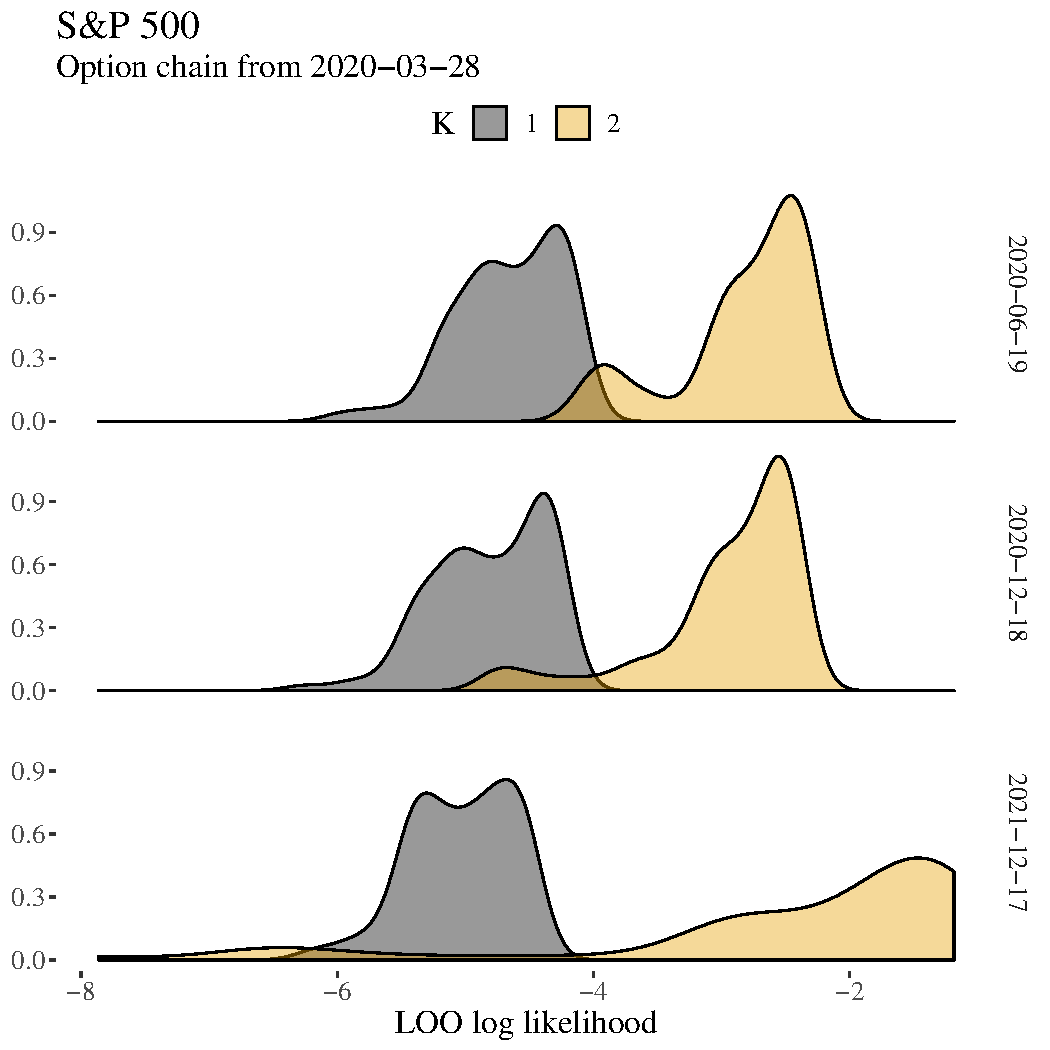
\includegraphics[width=0.95\textwidth]{model_loo.pdf}
  \end{center}
  \caption{Visual model comparison based on LOO log likelihood.}
\end{marginfigure}

\begin{figure}
  \begin{center}
    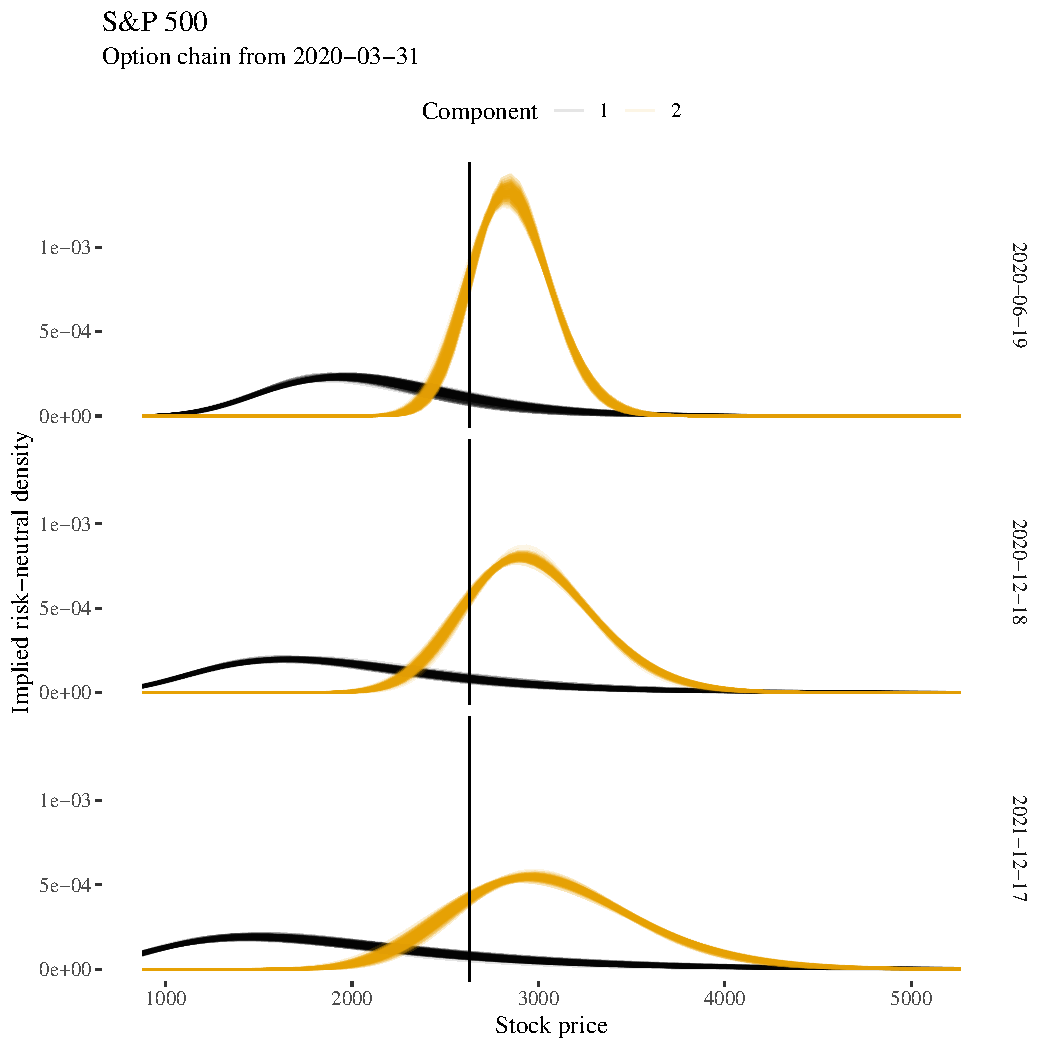
\includegraphics[width=0.95\textwidth]{risk_neutral.pdf}
  \end{center}
  \caption{Components of fitted implied risk-neutral density. Shown
    are 100 draws from the posterior distribution.}
\end{figure}

\begin{marginfigure}
  \begin{center}
    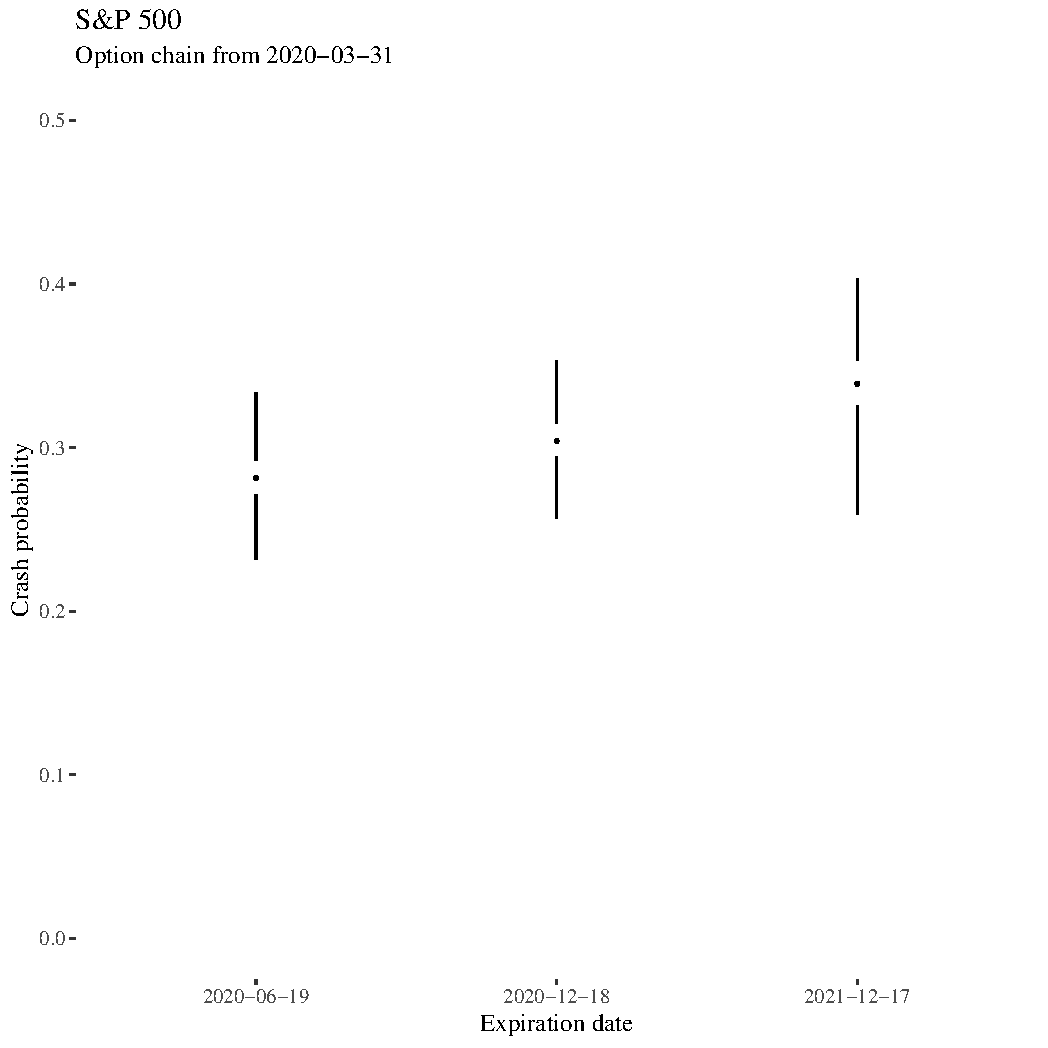
\includegraphics[width=0.95\textwidth]{crash_prob.pdf}
  \end{center}
  \caption{Market implied crash probability derived from two component
    mixture model.}
\end{marginfigure}

\end{document}
